\chapter{Summary and Outlook}

\section{Conclusions}

We have successfully developed an \insilico\ modeling protocol which accurately and efficiently predicts RI values of organic polymeric materials. This has also demonstrated its superior performance by faithfully reproducing the experimentally known RI values of 112 compounds. We have benchmarked DFT approaches for calculation of polarizability, which require RI calculations as an input. Our work provides an example of the synergistic benefits of fusing physical and data models. Furthermore, it is a clear embodiment of the promising nature of machine learning and modern data science in chemical research.

We utilized this new RI protocol to conduct virtual high-throughput screening studies on large-scale candidate libraries to discover novel organic polymers with high RI values. We demonstrated that computational modeling can rapidly and efficiently assess the properties and performance potential of candidate compounds. By combining our RI prediction model with virtual high-throughput screening techniques, we characterized polyimide candidates on a massive scale. We identified design rules as well as high-value building blocks, and structural patterns that correlate with the RI values. Additionally, we identified regions in the chemical space where we can maximize the RI values of organic polymers. These guidelines allow us to target specific molecular motifs and create next-generation polymers with exceptional optical properties. 

Using our in-house molecular library generator, \chemlg, we have generated a molecular library of 1.5 million small organic molecules. We performed DFT and MD simulations on a subset of this library, 100,000 compounds, to evaluate their polarizability and packing density values, respectively. By using the data from these simulations as a training set, we developed exceedingly efficient neural network models to correlate molecular structural descriptors with the target properties. Application of neural network models resulted in the acceleration of the property prediction of 1.5 million molecules. We mined this huge data and obtained insights into the correlation between the molecular structure and density of materials. Additionally, we evaluated the learning curve for the density prediction to obtain a correlation between the model efficiency and size of the data. We performed a similar analysis for the polarizability values, thus, allowing us to identify targets that can maximize the optical properties. 

The developed rational design framework is a powerful tool and has shown to be highly promising for rapidly identifying molecular candidates with exceptional RI values as well as discovering design rules for advanced materials. This dissertation serves as a proof-of-principle for our software ecosystem, which recognizes the great opportunities that are appearing with the shift towards a data-driven \insilico\ research paradigm in chemistry, materials science, and the corresponding engineering disciplines. We have shown \via\ this project that this approach indeed offers a path to overcome some of the prevalent limitations of traditional trial-and-error approaches. Our aim is to extend the capabilities of our cyberinfrastructure to tackle complex discovery and design challenges, increase the rate and quality of innovation, improve our understanding of the associated molecular and condensed matter systems, and democratize the tools that make these developments possible. The long-term objective of our work and related efforts by others is to help pioneer a fundamental transformation of the discovery process in chemistry, to make data science an integral part of the chemical enterprise, to shape the transition towards a data-driven discovery and rational design paradigm, and to spearhead a broad move by the community along those lines.

\section{Challenges for Organic Materials in Optical Applications}

In addition to the RI property, it is also very important to evaluate other optical properties such as transparency, Abbe number, and birefringence.

\begin{itemize}
	\item\textbf{Optical transparency:} Although most of the highly polarizable moieties increase the RI of the organic polymers, it is possible that the optical transparency of the material is affected. For example, in case of the polyimides, there is a possibility of formation of intermolecular charge-transfer complexes leading to the coloration of the material \cite{Takasaki2000}. The complexes are formed due to the charge transfer between electron accepting dianhydride and electron accepting diamine moiety. Thus, overcoming this trade-off between the optical transparency and RI is crucial.

	\item\textbf{Abbe number:} The high RI polymers that are being developed by incorporating highly polarizable moieties typically have low Abbe numbers. Abbe number is inversely proportional to the optical dispersion and therefore materials having low Abbe numbers will have high optical dispersions. Such materials are generally not preferable in optical devices because of reduced chromatic aberration \cite{Robello2013}. One of the approaches for improving the Abbe number is to include saturated moieties into the polymer as a side chain \cite{Takano2010}. For example, a compact and saturated structure like diamondoid can be incorporated as a side chain to tune the Abbe number of the polymer \cite{Namikoshi2014}. Diamondoids not only increase the Abbe number, but as they have high molar refraction they also concomitantly increase the RI of the polymers \cite{Robello2013,Gunawan2014}. However, the RI of these polymers is not quite high to be used in optical applications where high ($>$1.7) RI materials are required. Thus, it a challenging topic to optimize the structure of the polymers that have both high RI and high Abbe number values.

	\item\textbf{Birefringence:} Another vital property that should be considered in developing organic optical polymers is the birefringence parameter. If a material has high birefringence value, the polarization state of the incident light can be degraded resulting in a poor performance of the optical device, hence it is critical to consider the birefringence when designing materials for optical devices. The method of developing high RI polymers by introducing highly polarizable moieties often also results in the polymers with high birefringence. Thus, it is a challenge to design polymers having high RI and at the same time having low birefringence.  Numerous efforts are being made to lower the birefringence of organic polymers.  Recently, it was reported that polyamides show lower birefringence compared to polyimides while both have similar RI \cite{Javadi2013}. Quite recently, Seto \etal have attempted to develop aromatic polyesters and polycarbonates which are shown to have low birefringence along with having moderately high RI \cite{Seto2010}. Although these polymers have very attractive birefringence values, the RI of these polymers is still not high enough for optical applications. Further improvement of the RI of such polymers while keeping low birefringence is possible by optimizing the structure of the polymers in a favorable fashion.
\end{itemize}

Cross-linked structures (hyper-branched polymers): 
Many optical applications not only require materials with superior optical properties but also need them to have good mechanical integrity. Cross-linking of polymer networks has shown to increase the mechanical stability of the polymer materials \cite{Griebel2014,Bhagat2012,Mosley2014,Lin2010a,Jim2009a}. It has been observed that the cross-linking of high RI polymers concomitantly results in a further increase of RI \cite{Griebel2014}. In addition to this, cross-linking can also result in materials that have high optical transparency, low optical dispersion, low birefringence, and increased thermal stability \cite{Jim2009a,Lin2010a}. For example, a very recent study suggests that the cross-linked phenylthiophenyl silicone structures not only showed high RI values but also exhibited high thermal stability \cite{Mosley2014}. Thus, developing cross-linked polymer networks can lead to materials with very promising properties such as good mechanical and thermal stability along with high RI, low birefringence, high optical transparency and low optical dispersion. 

Recently, Bhagath et al. reported high RI thiol-ene polymers which have high packing density \citep{Bhagat2012,Bhagat2015,Bhagat2017,Bhagat2018}. The RI of these polymers was increased by incorporating functional moieties like aromatic groups, sulfur and other highly polarizable atoms like Si and Sn as shown in Fig.\ \ref{fig:thiol-ene}. These polymers show high RI ($>$1.7) as well as have very good mechanical strength. Further, the processing of these polymers is relatively easier compared to other polymers. We performed a few preliminary studies on these polymers (see App. \ref{appendix:B}). Our plan for the future is to apply our materials discovery framework to discover new thiol-ene polymers with exceptional RI values.

\begin{figure}[htbp]
	\centering
	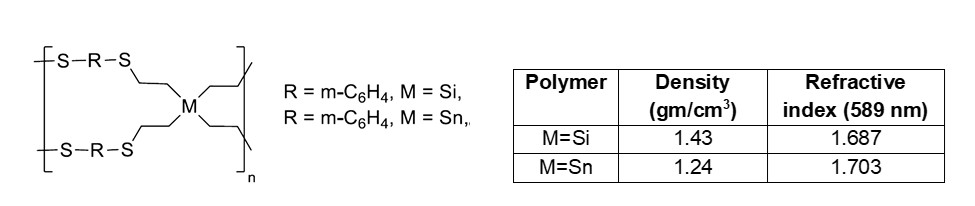
\includegraphics[width=1.00\textwidth]{Chapter-7/Figures/thiol-ene.jpg}
	\caption{Thiol-ene polymers with high packing density and high RI \cite{Bhagat2012}.}
	\label{fig:thiol-ene}
\end{figure}

\section{Improving our Cyberinfrastructure}
 
We are currently working on the following aspects of our cyberinfrastructure to further improve its applicability:

\begin{itemize}
	\item \chemlg: The library generator currently implements the genetic algorithm for linear molecules. Ongoing work in this area aims to extend this algorithm to traverse molecules in multiple dimensions. Further, we plan to implement other smart algorithms such as Monte Carlo search and Simulated Annealing. 
	\item \chemhtps: Currently, \chemhtps\ is setup to run on SLURM queuing systems. We plan to extend \chemhtps\ to other queuing systems such as PBS. It currently supports the ORCA \cite{Neese2012}, Q-Chem \cite{Shao2014}, and GROMACS \cite{ABRAHAM201519} modeling packages, and bindings to other quantum chemistry, molecular dynamics, and solid state physics codes are planned for the future.
	\item \chembddb: The future work in \chembddb\ includes the integration of external databases to extract information on existing molecules or obtain data using cheminformatics from the websites such as ChemSpider. 
	\item \chemml:  We plan to extend \chemml\ capabilities by implementing new advances in machine learning, such as convolutions, transfer learning, active learning, and reinforcement learning. Mojtaba Haghighatlari is taking a lead on adding these functionalities as well as applying them to improve the packing density, polarizability, and RI prediction models
\end{itemize}

In addition to implementing new algorithms and extending our cyberinfrastructure's applicability, we continuously focus on the ease of use, workflow, and code integration to make this technology more accessible to the community.